\SACCMD{image}
\label{cmd:image}

\SACTitle{概要}
利用内存中的数据文件绘制彩色图

\SACTitle{语法}
IMAGE [ COLOR | GREY ] [ BINARY|FULL ] [ PRINT [ pname ] ]

\SACTitle{输入}
\begin{itemize}
\item COLOR|GREY :  绘制彩图或者灰度图
\item BINARY|FULL :  绘图时所有正值是一个颜色,所有负值是另一种颜色,或者根据数据值不同变换颜色 
\item PRINT pname : 将输出图形打印到打印机 
\end{itemize}

\SACTitle{缺省值}
IMAGE COLOR FULL

\SACTitle{说明}
这个命令允许用户根据SAC三维数据绘制彩图或灰度图,三维数据一般由spectrogram,scallop或bbfk命令产生,你也可以导入自己生成的SAC格式三维数据。可以使用xlim和ylim查看图形的不同区域,也可以通过一位操作符修改幅度

\SACTitle{例子}
以\${SACHOME}/macros/data/contourdata作为例子:
\begin{SACCode}
SAC> r contourdata
SAC> image
\end{SACCode}

\begin{figure}[h]
\centering
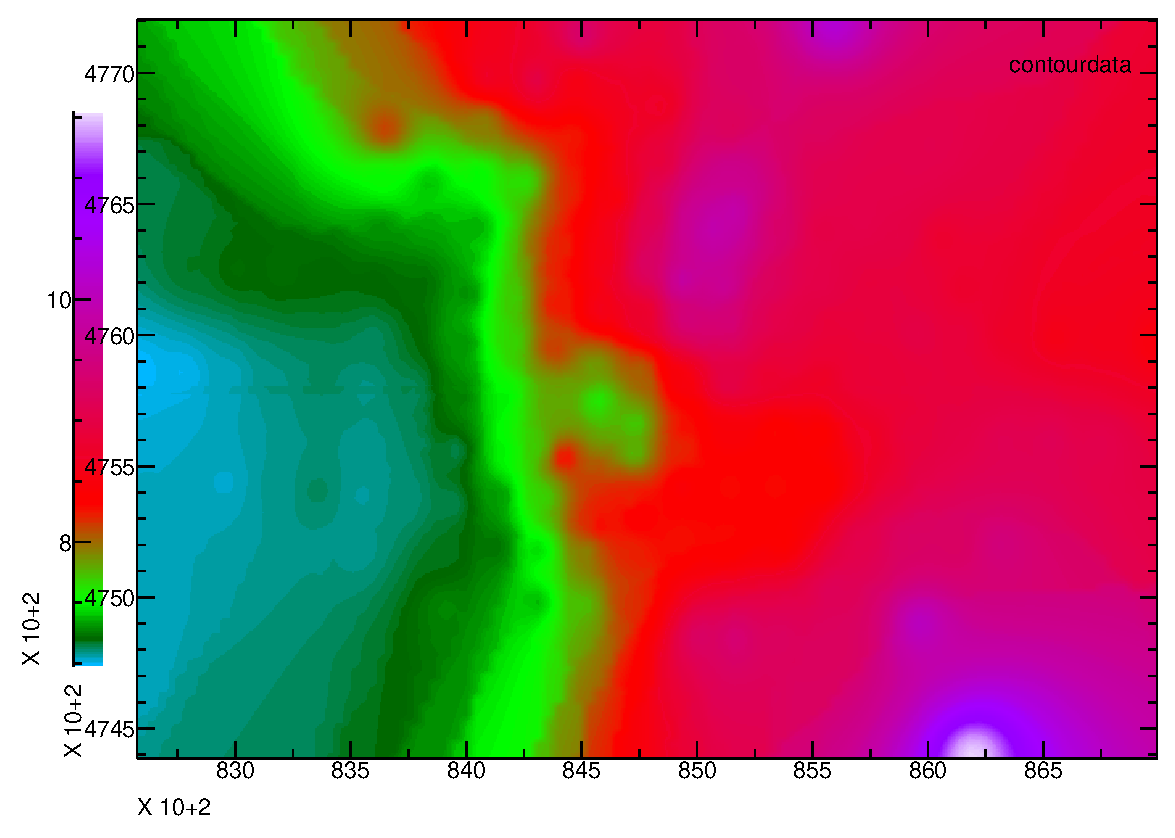
\includegraphics[width=14cm]{image}
\caption{IMAGE例子示意图}
\end{figure}

\SACTitle{头段变量}
需要:  IFTYPE (设为``IXYZ''), NXSIZE, NYSIZE

使用:XMINIMUM, XMAXIMUM, YMINIMUM, YMAXIMUM

\SACTitle{最近修订}
May 26, 1995 (Version 00.31)
